%%
%% Copyright 2007, 2008, 2009 Elsevier Ltd
%%
%% This file is based on part of the 'Elsarticle Bundle'.
%% ---------------------------------------------
%%
%% It may be distributed under the conditions of the LaTeX Project Public
%% License, either version 1.2 of this license or (at your option) any
%% later version.  The latest version of this license is in
%%    http://www.latex-project.org/lppl.txt
%% and version 1.2 or later is part of all distributions of LaTeX
%% version 1999/12/01 or later.
%%
%% The list of all files belonging to the 'Elsarticle Bundle' is
%% given in the file `manifest.txt'.  Contact Elsevier for this file.
%%

%% Template article for Elsevier's document class `elsarticle'
%% with harvard style bibliographic references
%% SP 2008/03/01 
%%
%% $Id: elsarticle-template-harv.tex 4 2009-10-24 08:22:58Z rishi $
%%
%% This template is based on the 'elsarticle-template-harv.tex', but has been modified for specific use with submissions to the journal Ultrasound in Medicine and Biology, June 2010, KJH
%%

% Use this set of document class options for submission
\documentclass[preprint,5p,authoryear]{elsarticle}

% Use this set of document class options to obtain an approximate 2 column view, note that this is primarily intended to allow authors to determine line breaks for long equations.  It is NOT meant to identically reproduce how the article would look in print.
%\documentclass[3p,twocolumn,authoryear,12pt]{elsarticle}


%% if you use PostScript figures in your article
%% use the graphics package for simple commands
%% \usepackage{graphics}
%% or use the graphicx package for more complicated commands
%% \usepackage{graphicx}
%% or use the epsfig package if you prefer to use the old commands
%% \usepackage{epsfig}

%% The amssymb package provides various useful mathematical symbols
\usepackage{amssymb}
%% The amsthm package provides extended theorem environments
%% \usepackage{amsthm}

%% The lineno packages adds line numbers. Start line numbering with
%% \begin{linenumbers}, end it with \end{linenumbers}. Or switch it on
%% for the whole article with \linenumbers after \end{frontmatter}.
 \usepackage{lineno}
 
 %% The multirow package adds the ability to do multirow and 
 %% multicolumn spanning in LaTeX.  This package is used 
 %% as an example for this template in the tables section.
 \usepackage{multirow}
 \usepackage{graphics}
 \usepackage{float}
 \usepackage{graphicx}% http://ctan.org/pkg/graphicx

\journal{Ultrasound in Medicine and Biology}

\begin{document}

\begin{frontmatter}

%% Title

%% use the tnoteref command within \title for footnotes;
%% use the tnotetext command for the associated footnote;
%%
%% \title{Title\tnoteref{label1}}
%% \tnotetext[label1]{}
%% \author{Name\corref{cor1}\fnref{label2}}
%% \ead{email address}
%% \ead[url]{home page}
%% \fntext[label2]{}
%% \cortext[cor1]{}
%% \address{Address\fnref{label3}}
%% \fntext[label3]{}

\title{Acoustic Shadow Detection: Study and Statistics of B-Mode and Radiofrequency Data}


%% Authors and addresses/affiliations

%% use the fnref command within \author or \address for footnotes;
%% use the fntext command for the associated footnote;
%% use the corref command within \author for corresponding author footnotes; note the corresponding author can be any of the authors, but one author must be designated; here the third author has been arbitrarily designated as the corresponding author as an example.
%% use the cortext command for the associated footnote;
%% use the ead command for the email address,
%% and the form \ead[url] for the home page:

%% \author{Name\corref{cor1}\fnref{label2}}
%% \ead{email address}
%% \ead[url]{home page}
%% \fntext[label2]{}
%% \cortext[cor1]{}
%% \address{Address\fnref{label3}}
%% \fntext[label3]{}

%% use optional labels to link authors explicitly to addresses:
%% \author[label1,label2]{<author name>}
%% \address[label1]{<address>}
%% \address[label2]{<address>}

\author[Affil1]{Ricky Hu \corref{cor1}}
\author[Affil1]{Rohit Singla}
\author[Affil1]{Farah Deeba}
\author[Affil1][Affil2]{Robert N. Rohling}

\address[Affil1]{Department of Electrical and Computer Engineering, University of British Columbia, Vancouver, Canada}
\address[Affil2]{Department of Mechanical Engineering, University of British Columbia, Vancouver, Canada}
% Replace capitalized text with the appropriate information (use standard capitalization rules for your text, not all capitals.
\cortext[cor1]{Corresponding Author: Ricky Hu, Robotics and Control Laboratory, University of British Columbia, Room 3090, 2332 Main Mall, Vancouver, BC, Canada V6T 1Z4.  Email: rhu@ece.ubc.ca}


\begin{abstract}
	An acoustic shadow is an ultrasound artifact occurring at boundaries between significantly different materials, resulting in a continuous dark region on the image. Shadow detection is important as shadows can identify anatomical features or obscure regions of interest. A study was performed to scan human subjects (N=35) specifically to explore the statistical characteristics of various shadows from different anatomy and with different transducers. Differences in shadow statistics were observed and used for shadow detection methods with radiofrequency (RF) or brightness-mode (B-mode). Both methods utilized adaptive thresholding, needing only the transducer pulse width as an input parameter for easy utilization by different operators or equipment. Mean Dice coefficients ($\pm$ standard deviation) of 0.90$\pm$0.07 and 0.87$\pm$0.08 were obtained for the RF and B-mode methods, which is within range of manual annotators. The results indicate that the methods are able to detect shadows with high versatility in different imaging scenarios. The understanding of shadow statistics can be used for more specialized methods can be developed for specific applications in the future. The detection methods can also potentially aid interpretation of ultrasound images or serve as an important pre-processing step for machine learning methods. 
\end{abstract}


\begin{keyword}
	%% keywords here, in the form: keyword \sep keyword.  You may use no more than 10 keywords.
	Acoustic Shadow \sep Ultrasound \sep Speckle \sep Radiofrequency \sep Segmentation
\end{keyword}

\end{frontmatter}

%% Do not remove the page break here.
\pagebreak

\linenumbers

%% MAIN TEXT INSTRUCTIONS

%% For all sections, subsections, and subsubsections, use the '*' to remove numbering, as demonstrated below.

%% Commands for figures and tables should not be included in the main body of the submitted version of this file (e.g. the figure and tabular environments).  Figure captions should be listed in this file, as shown below.  Tables and Table captions should be listed as a separate section at the end of this file, as shown below.  Many authors may wish to include figures and tables within the main text of their document will preparing their manuscript.  This may be done, however please comment out any of the lines prior to submission.

%% Because the Elsevier editorial process does not allow for the figure and tabular environments in the submitted document, you will be unable to use autonumbering (i.e. \label and \ref) for figures and tables. 

%%  If long equations are used in the document, authors should use a two column format to make sure that the equations will break at approximately the right places.  To do this, replace the class option 'review' with the following two class options '3p' and 'twocolumn'.  Keep in mind that the column width produced in '3p' is slightly narrower than the final printer version.  After inserting the appropriate line breaks in your equation, change the '3p' option back to 'review'.

%% For citations, use the commands \citep and \citet

%% BEGIN MAIN TEXT

%%%%%%%%%%% INTRODUCTION
\section*{Introduction}
\label{intro}
Ultrasound devices have become increasingly affordable and portable, encouraging applications such as point-of-care ultrasound \citep{Bouhemad2011}, novice usage \citep{Sippel2011}, and analysis by machine learning \citep{Ghose2013}. However, ultrasound is susceptible to unique artifacts that increase the difficult of interpretation and processing of images. One artifact is an acoustic shadow, which occurs when an ultrasound wave crosses a boundary of two materials with high impedance differences \citep{Kremkau1986}. The wave is almost completely reflected and depicted beyond the boundary is a continuous dark region and a loss of anatomical features. Shadows occur in air-tissue, tissue-bone, and tissue-lesion interfaces. Shadows can aid interpretation, such as identifying gall stones \citep{Good1979} or spinal levels \citep{Galiano2005}. However, shadows, such as from poor transducer contact, can lead to misinterpretation of anatomy, particularly by novice users and automated processing algorithms. Thus, the identification of shadows is an important preprocessing step in many applications.

Several methods have been used in literature to detect shadows and illustrative examples are discussed. Geometric techniques model the path of an ultrasound signal for an expected image along the scanline using a random walk \citep{Karamalis2012}. Pixels are then flagged as a shadow if it is below a confidence threshold. However, geometric techniques require knowledge of ultrasound transducer properties to parameterize random walk weights, such as the focal length, radius of curvature, and thickness. The technique is more cumbersome to implement across different ultrasound machines. This also reduces applicability for machine learning applications as accurate transducer parameter labels are required for each image.

Pixel intensity methods ignore the transducer properties and analyze only the graphical properties of animage \citep{Hellier2010}. Shadows have been detected on brain images by analyzing the entropy along a scanline to flag pixels of sudden low entropy as a potential shadow. The technique achieved a comparable Dice similarity coefficient as geometric methods but require specific thresholding, window sizing, filtering, and image mask parameterization for different anatomy and transducers. The drawback is that parameterization requires image processing expertise, infeasible in novice point-of-care applications.

Machine learning methods have gained significant interest in medical imaging analysis. To our knowledge, no machine learning method has demonstrated capability of general shadow detection from multiple anatomy. Deep learning methods have identified features in a specific image sets that contain shadows, such as neuroanatomical regions in cranial scan \citep{Milletari2017} or spinal levels in a posterior scan \citep{Hetherington2017}. Although machine learning has the potential of providing automated feature recognition in multiple applications, a large data set is required for an algorithm to recognize certain features. Ultrasound imaging is highly variable due to unique artifacts, operator technique, and equipment. In addition, shadows are a very general feature that occur in various imaging scenarios. Previous techniques focus on a single anatomical region and training data was from a consistent imaging scenario. However, it is difficult to construct a training data set with the generality required to recognize shadows in different scenarios usable for a variety of ultrasound applications.

There are two objectives to this paper. First, to address the need for understanding general characteristics of shadows, a study was conducted to scan multiple anatomy and transducers specifically to analyze the statistics of different types of shadows. Second, to address existing needs for versatile detection with minimal parameterization, previous methods were then extended utilizing statistical thresholding of radiofrequency (RF) or brightness-mode (B-mode) data to detect shadows from various imaging scenarios. 

%%%%%%%%%%% MATERIALS AND METHODS
\section*{Materials and Methods}
\label{MaM}
\subsection*{Data Collection}
Ultrasound RF and B-mode data was acquired by scanning 37 adult participants with informed written consent, approved by the University of British Columbia Research Ethics Board (Study ID: H18-01199). The scans included a forearm scan near the distal end of the pronator quadratus, an elbow scan near the cubital fossa, and a rib scan on the anterior surface of right ribs 11-12. Each scan was taken with both a curvilinear (C5-2/60, Ultrasonix, Canada) and linear (L14-5/38, Ultrasonix, Canada) transducer. Different transducer settings were used for each anatomical region and transducer, summarized in Table 1. Shadows are expected to occur due to superficial and deep bones and from an air gap created by the lateral edges of the transducer not being in flush contact with the skin. The experiment was designed to generate a dataset from various imaging scenarios to explore general shadow characteristics and to validate the versatility of the shadow detection methods. 

\subsection*{Radiofrequency Speckle Analysis}      
To analyze shadows, windows of speckle were analyzed on the RF signal. Speckle occurs due to multiplicative scattering of acoustic waves in a material, resulting in a granular appearance on the image. The benefit of RF analysis is that B-mode image processing commonly attempts to remove speckle, but speckle contains information of the acoustic interactions in tissue \citep{Burckhardt1978}. Speckle can then characterize different regions, such as a region of tissue or a region of signal loss in a shadow. In addition, B-mode image formation can be manipulated by an operator to visually enhance an image, such as adjusting time-gain compensation or dynamic range. Thus, the underlying speckle analysis can provide shadow detection usable across different machines and operators.

One of the first models for speckle is with a one parameter Rayleigh distribution to model the probability density of a random walk \citep{Burckhardt1978}. The Rayleigh distribution is capable for modeling fully developed speckle, which does not occur in limited scattering \citep{Tuthill1988}. More generalized models have been applied such as the Rician, Homodyned-K, and Nakagami distributions to characterize speckle \citep{Destrempes2010}. The utility of speckle has been demonstrated in the literature to classify tumorigenicity of breast lesions \citep{Byra2016} or levels of liver fibrosis \citep{Ho2012} by categorizing image regions based on the speckle pattern. Shadow characterization presents a simpler problem as a shadow and non-shadow region contain significantly different speckle patterns. Thus, the Nakagami distribution expressed in Eq. 1 was chosen to model speckle. The Nakagami distribution provides greater generality than the Rayleigh distribution while being more computationally efficient than the Rician or Homodyned K distributions \citep{Destrempes2010}.

\begin{equation}
\Phi(x,\mu,\omega) = 2(\frac{\mu}{\omega})^{\mu}\frac{1}{\Gamma(\mu)}x^{(2\mu-1)}e^{\frac{-\mu}{\omega}x^{2}}
\end{equation}

where $x$ is RF intensity, $\mu$ is a shape parameter, $\omega$ is a scale parameter and $\Gamma(\mu)$ is the gamma distribution.

To characterize shadows, the raw RF data was first processed by computing the echo envelope of each scanline with a Hilbert transform. This creates a pre-scan converted image, visually similar to B-mode but without filtering to remove speckle. Next, the RF image was divided into overlapped windows with a width of a single RF data point and a length of three times the pulse width. This patch size was demonstrated in literature to be sufficiently large to capture multiple wavelengths and scattering events while being small enough to be useful in differentiating different regions on the millimeter scale \citep{Byra2016}. Next, each window was fit to a Nakagami distribution using a maximum likelihood estimate to compute a map of Nakagami parameters $\mu$ and $\omega$, as shown in Fig. 1.

To detect shadows, Otsu's method was applied on the entire image to automatically compute a threshold for the $\omega$ parameter. This was sufficient as the $\omega$ parameter is significantly different for shadow regions with abundant speckle and non-shadow regions with minimal speckle, Then, for each scanline, the axially deepest data point that is above the threshold is labeled as the shadow boundary and all data points below are labeled as a shadow.

\subsection*{B-mode Scanline Analysis}

Many ultrasound machines do not provide access to RF data for speckle analysis. Thus, a previous pixel-intensity shadow detection method on B-mode images was modified and extended. Scanline entropy was investigated on B-mode images to characterize different types of shadows, but with the addition of adaptive thresholding of entropy to address the need for usability with minimum configuration. First, the cumulative scanline entropy is computed for each pixel, similar to the ``Rupture Criterion" \citep{Hellier2010}, with the window size fixed as three times the pulse width, $\eta$, as defined in Eq. 2. For the case of curvilinear images, radial scanlines were linearly interpolated between the two symmetric lateral edges of the image.

\begin{equation}
S_{i,j} = \sum_{i=1}^{3\eta}I(i-1)log_{2}\frac{I(i-1)}{I(i+1)}+I(i+1)log_{2}\frac{I(i+1)}{I(i-1)}
\end{equation}

where $S_{i,j}$ is the cumulative entropy at pixel $i$ on scanline $j$, $\eta$ is the pulse width, and $I(i)$ is the pixel intensity of $i$.

Next, Otsu's method is applied similarly to compute a threshold entropy value. The intuition of the threshold is different than in RF analysis. In RF analysis, the threshold separates patches of intense and minimal speckle. In B-mode analysis, the threshold separates pixels of a shadow boundary, which has high entropy, and pixels away from shadow boundary, which include shadow and non-shadow regions. Thus, shadows can be identified by finding the last pixel on a scanline with an entropy higher than the threshold, representing a bright shadow boundary.


\subsection*{Validation}

A trained annotator (RH) manually outlined shadow regions on B-mode images. The manual regions were used as a gold standard, as manual identification is common in clinical practice and has been used in previous literature for comparison \citep{Hellier2010}. A Dice coefficient was computed to compare similarity of manual and automated shadow detection. The manual outline was used to define four regions for classification of statistical parameters: a non-shadow region above the boundary, a shadow region below the boundary, and a ``transition region", which is a window defined as three pulse widths long axially centered at shadow boundary.
%
%%%%%%%%%%% Results
\section*{Results}
\label{Results}
Examples of detected shadows from both methods are highlighted in gray in Fig. 2 in different imaging scenarios. The Dice coefficients for both methods for different anatomy and transducers are shown in Table 2. The mean Dice coefficients ($\pm$ standard deviation) were 0.90$\pm$0.07 and 0.87$\pm$0.08 for RF and B-mode methods. Manual annotation was repeated five times with a mean Dice coefficient of 0.92$\pm$0.02 for all images and transducers.

With the benefit of a varied dataset, general characteristics of shadows can be analyzed, as summarized in Table 3. The log-scale Nakagami $\omega$ parameter recorded a mean $\pm$ standard deviation of $13.95\pm2.03$ for all non-shadow and $8.89\pm1.16$ for shadow regions defined by manual outlining of all images. The $\mu$ parameter recorded $1.02\pm0.29$ for non-shadow and $3.25\pm2.35$ for shadow-regions.  TALK ABOUT ENTROPY HERE.


%%%%%%%%%%% DISCUSSION
\section*{Discussion}
\label{Discuss}
The RF and B-mode shadow detection developed achi-eved a high Dice similarity coefficient for all anatomy and transducer types. Previous studies reported that the Dice coefficient between manual annotators recorded a mean of 0.91$\pm$0.07 \citep{Hellier2010}. Every scenario detected from both methods achieved a Dice coefficient within the range of manual detection within operator variability. An important feature of shadow detection is being able to differentiate between a shadow and simply high attenuation of the signal. Both scenarios result in an eventual loss of signal. Shadow detection, however, has a characteristic high intensity shadow boundary before a significant loss in signal, compared to gradually signal losses in attenuation. Both methods were capable of this distinction. The high accuracy supports the versatility of the detection method as both methods are able to identify shadows across different anatomy and transducers with minimum configuration. 

For a general observation for shadows, the computed Nakagami $\omega$ parameter of all manually outlined shadows indicate that there is a statistically significant difference between shadow and non-shadow regions, even with the error in the transition regions considered. The speckle from shadows is thus distinct from the speckle created by tissue, muscle, or fat. This is likely due to shadows representing a region where almost no acoustic speckle interactions occur as the waves have been reflected at a preceding boundary.  


In RF detection, both false positive and false negative errors most frequently occurred immediately below a shadow boundary as opposed to B-mode detection where errors were in various regions. The Nakagami distributions in patches near the boundary resemble distributions for non-shadows. Moreover,  granular RF speckle can be visually observed in a neighborhood around a boundary. The speckle gradually lessens after a brightest point on a scanline, possibly due to incomplete total reflection at a boundary. This indicates that the boundary is not an instantaneous division between non-shadow and shadow, rather, there is a ``transition region" before the image fully resembles a shadow with a loss of signal. This is quantified by the statistics of the speckle in the transition region, where deep shadows were observed to have a significantly different Nakagami distribution than non-shadows, but transition regions were much more similar to non-shadows.

In previous literature, shadows were defined qualitatively \citep{Kremkau1986} as a sudden loss of signal and brightness. The observed transition region in this study suggests that the qualitative definition of a shadow may be insufficient for accurate detection. One algorithm may detect the shadow starting immediately after the brightest location, or another may use a convention such as a full width at half maximum to define where the signal has sufficiently low intensity to resemble the start of a shadow. There is a decision point required for a clear definition for where a shadow begins to improve shadow detection accuracy, both from a signaling perspective for image processing and a visual perspective for manual inspection. 


The findings in this study result in several implications. First, the statistics of acoustic shadows have been investigated on a dataset with shadows occurring from multiple scenarios as opposed to specific cases where shadows are observed. This provided a more generalizable observation that shadows can be characterized by speckle distributions and that there exists a transition region before the loss of speckle in a shadow. Second, the shadow detection methods demonstrated high accuracy, indicating that accurate shadow detection is possible regardless of transducer or imaging location. In future studies, the speckle statistics observed can be used to develop further models for anatomical features containing shadows, such as training a machine learning algorithm to measure the size of gall stones. Future studies would also have to take into consideration the most frequent source of error of shadow detection as the shadow boundary. For instance, a convention can be develop for one algorithm to detect the surface of the gallstone as the brightest point on a scanline to be comparable with other images.

%%%%%%%%%%% Conclusions
\section*{Conclusions}
\label{Conclusions}
Acoustic shadows from different imaging scenarios were investigated. RF and B-mode methods were developed for acoustic shadow detection requiring only the transducer pulse width as the input parameter. When comparing to manual detection, the methods achieved a Dice similarity coefficient within range of manual observers. The work focused on applying shadow detection and statistical analysis to a varied dataset of three different anatomical locations and two different transducer to provide a representative understanding of general acoustic shadows. The statistics of acoustic shadow indicate that shadows contain a distinct speckle distribution compared to non-shadows and the speckle characteristics transition at the shadow boundary. The statistical findings of shadows can aid interpretation of ultrasound images in the future using speckle analysis. The versatility of the shadow detection method has the potential to improve the interpretation of ultrasound images with shadow artifacts or to serve as a pre-processing step for machine learning methods.

        
%%%%%%%%%%% ACKNOWLEDGEMENTS
\section*{Acknowledgements}
\label{Ack}
This work is supported by the National Sciences and Engineering Research Council of Canada.



%% The Appendices part is started with the command \appendix;
%% appendix sections are then done as normal sections
%% \appendix

%% \section*{}
%% \label{}


%%%%%%%%%%% REFERENCES
%% REFERENCE FORMATTING INSTRUCTIONS

%% All bibliography information should be included using a 'thebibliography' environment.  Most authors will find it easiest to create a .bbl file using the commands \bibliographystyle{} and \bibliography{} and then copy and paste the contents of the .bbl file into the .tex file below, but before the figure captions section.  Examples for using the \bibliographystyle and \bibliography commands are listed below.  

%% Do not remove the page break here.
\pagebreak

%% References with bibTeX database, use this to create a .bbl file
\bibliographystyle{UMB-elsarticle-harvbib}
\bibliography{bibliography}

%% References copied and pasted from the .bbl file.  Copy and paste over the following two lines.  When using a bibTeX database to create a .bbl file, comment out the following two lines.
%\begin{thebibliography}{00}
%\end{thebibliography}

%%%%%%%%%%% FIGURE CAPTIONS

%% Include only the figure captions here (not the figures).  Figures are uploaded separately in the online Elsevier Editorial Submission process.

%% Do not remove the page break here.
\pagebreak

\section*{Figure Captions}

\begin{description}
\item[Figure 1:]  A visualization of the B-mode and RF parameter maps. The b) Entropy Map was computed from processing of the a) original B-mode image and the d) Nakagami $\omega$ map was computed from the c) echo envelope. Note that the echo envelope contains noticeable speckle, which has been used to fit a Nakagami distribution to characterize shadow. The region at depth 2.50cm and scanlines 32-40 is attenuation and not a shadow. This is an important distinction in shadow detection and both maps show the region as below a threshold to flag a shadow boundary.
\item[Figure 2:]  A comparison of the original B-mode images, the detected shadows manual detection, RF detection, and B-mode detection. Both detection methods perform similar to manual detection. Both methods perform slightly less accurately on curvilinear images, likely due to the reduced resolution from interpolating the scanlines. Most errors of RF detection occur near the shadow boundary, likely due to the transitioning speckle from non-shadow to shadow.
\end{description}

\begin{figure}[H]
	\centering
	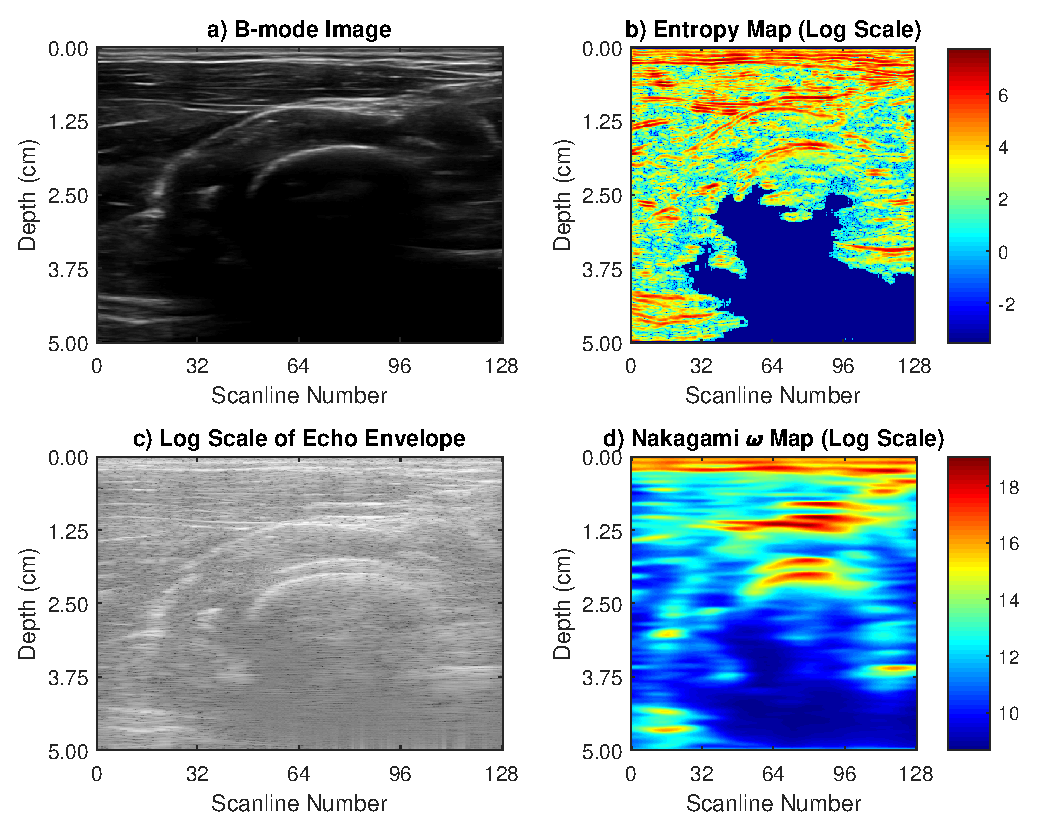
\includegraphics[scale=0.5]{fig2.pdf}
\end{figure}

\begin{figure*}
	\centering
	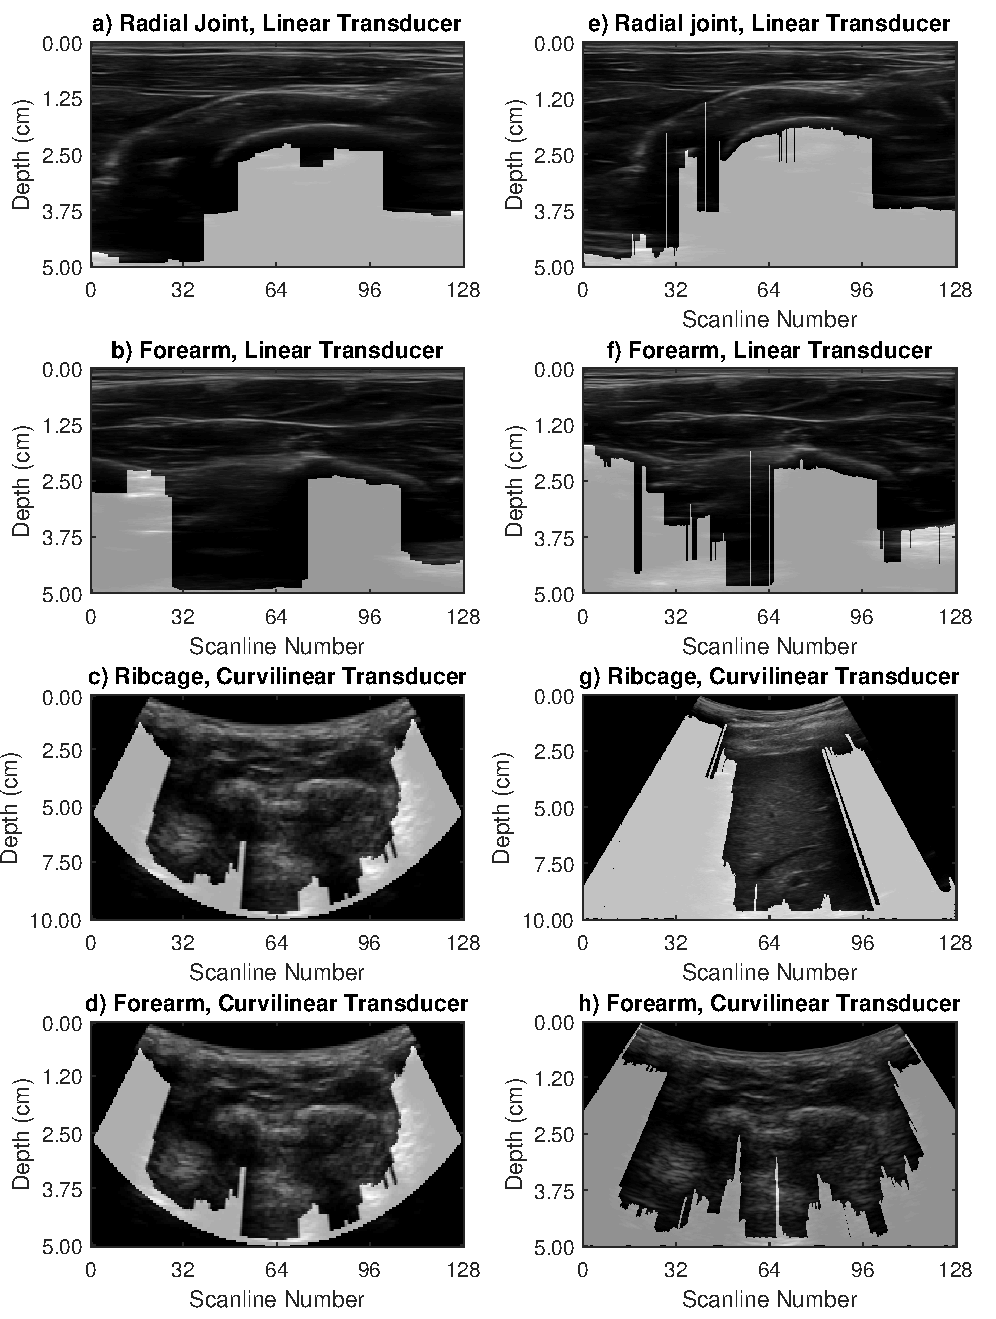
\includegraphics[scale=0.6]{fig1.pdf}
\end{figure*}

%%%%%%%%%%% TABLES AND TABLE CAPTIONS

%% Both tables and table captions should be included below.  Captions should appear above the table, as shown below. If users want to use multirow.sty, array.sty, etc., to fine control/enhance the tables, they are welcome to load any package of their choice and the elsearticle.cls should work in combination with all loaded packages.  For problems with loaded packages please contact: elsarticle@river-valley.com (the developers of the elsarticle document class) or support@elsevier.com (Elsevier customer support).

%% Since the tabular format is often difficult to work with for complex tables, authors may also choose to create their tables with another program.  Each table and it's corresponding caption should then be saved as a pdf.  Each pdf should then be uploaded separately during the online submission process.  If doing so, all of the text below concerning tables and table captions should be commented out.

%% If no tables are part of the manuscript, comment out or delete this entire section.

%% Do not remove the page break here.
\pagebreak

\section*{Tables}

\begin{description}
\item[Table 1:]  Transducer properties for different imaging scenarios. \\

\begin{table}[H]
	\begin{center}
		\resizebox{\columnwidth}{!}{
			\begin{tabular}{|l|l|l|l|l|}
				\hline
				\textbf{}                                                                                              & \textbf{Anatomy} & \textbf{Frequency} & \textbf{Depth} & \textbf{Gain} \\ \hline
				\multirow{3}{*}{\textbf{\begin{tabular}[c]{@{}l@{}}Linear\\ Transducer\\ (L14-5/38)\end{tabular}}}     & Forearm          & 11.0MHz            & 5.0cm          & 50\%          \\ \cline{2-5} 
				& Elbow            & 11.0MHz            & 5.0cm          & 40\%          \\ \cline{2-5} 
				& Ribcage          & 5.0MHz             & 10.0cm         & 30\%          \\ \hline
				\multirow{3}{*}{\textbf{\begin{tabular}[c]{@{}l@{}}Curvilinear\\ Transducer\\ (C5-2/60)\end{tabular}}} & Forearm          & 4.0MHz             & 5.0cm          & 50\%          \\ \cline{2-5} 
				& Elbow            & 4.0MHz             & 5.0cm          & 40\%          \\ \cline{2-5} 
				& Ribcage          & 3.3MHz             & 10.0cm         & 30\%          \\ \hline
		\end{tabular}}
	\end{center}
\end{table} 

\item[Table 2:]  Mean Dice coefficients for different imaging scenarios $\pm$ standard deviation. 


\begin{table}[H]
	\begin{center}
		\begin{tabular}{|l|l|l|l|}
			\hline
			\textbf{}                                                                                 &         & \textbf{RF} & \textbf{B-Mode} \\ \hline
			\multirow{3}{*}{\begin{tabular}[c]{@{}l@{}}Linear\\ (L14-5/38)\end{tabular}} & Forearm & 0.91$\pm$0.05                   & 0.89$\pm$0.06                             \\ \cline{2-4} 
			& Elbow   & 0.94$\pm$0.06                   & 0.90$\pm$0.07                             \\ \cline{2-4} 
			& Ribcage & 0.87$\pm$0.09                   & 0.84$\pm$0.06                             \\ \hline
			\multirow{3}{*}{\begin{tabular}[c]{@{}l@{}}Curvilinear\\ (C5-2/60)\end{tabular}}                                                  & Forearm & 0.89$\pm$0.05                   & 0.86$\pm$0.08                             \\ \cline{2-4} 
			& Elbow   & 0.93$\pm$0.04                   & 0.90$\pm$0.09                             \\ \cline{2-4} 
			& Ribcage & 0.83$\pm$0.08                   & 0.83$\pm$0.10                             \\ \hline
			\textbf{Mean}      & \textbf{All Anatomy} & \textbf{0.90$\pm$0.07}           & \textbf{0.87$\pm$0.08}               \\ \hline
		\end{tabular}
	\end{center}
\end{table} 
\end{description}

%%%%%%%%%%% VIDEO CAPTIONS

%% If submitting video's as a supplement to the manuscript, include only the video captions here (not the figures).  Videos are uploaded separately in the online Elsevier Editorial Submission process.  If videos are not included, comment out this section.

%% Do not remove the page break here.
\pagebreak

%\section*{Video Captions}
%
%\begin{description}
%\item[Figure 1:]  TYPE THE CAPTION FOR VIDEO ONE HERE.
%\item[Figure 2:]  TYPE THE CAPTION FOR VIDEO TWO HERE.
%\item[Figure 3:]  TYPE THE CAPTION FOR VIDEO ONE HERE.  CONTINUE THIS LIST FOR ALL OTHER CAPTIONS
%\end{description}
%


\end{document}
